%\section{CSU de EMIR}

%%%%%%%%%%%%%%%%%%%%%%%%%%%%%%%%%%%%%%%%%%%%%%%%%%%%%%%%%%%%%%
\begin{frame}
    \frametitle{CSU: Configurable Split Unit}
    \centering{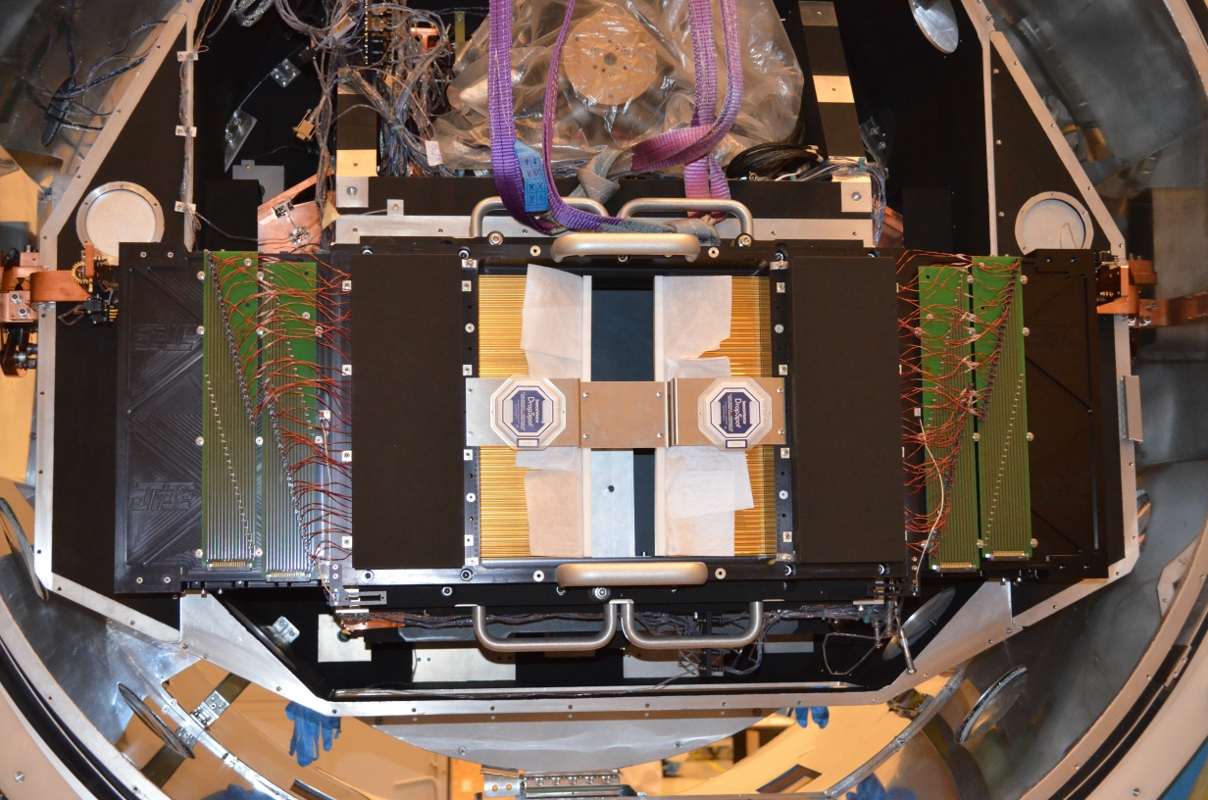
\includegraphics[width=0.8\linewidth]{FIGURES/DSC_0750}}
    \block{CSU}
    \begin{itemize}[<+->]
    \item Dimensiones $\rightarrow 240\times400$ arcosegundos
    \item 55 pares de barras
    \item Rotación
    \end{itemize}
    \endblock{}
\end{frame}
%%%%%%%%%%%%%%%%%%%%%%%%%%%%%%%%%%%%%%%%%%%%%%%%%%%%%%%%%%%%%%

%%%%%%%%%%%%%%%%%%%%%%%%%%%%%%%%%%%%%%%%%%%%%%%%%%%%%%%%%%%%%%
\begin{frame}
    \frametitle{Apuntado - Representación gráfica}
    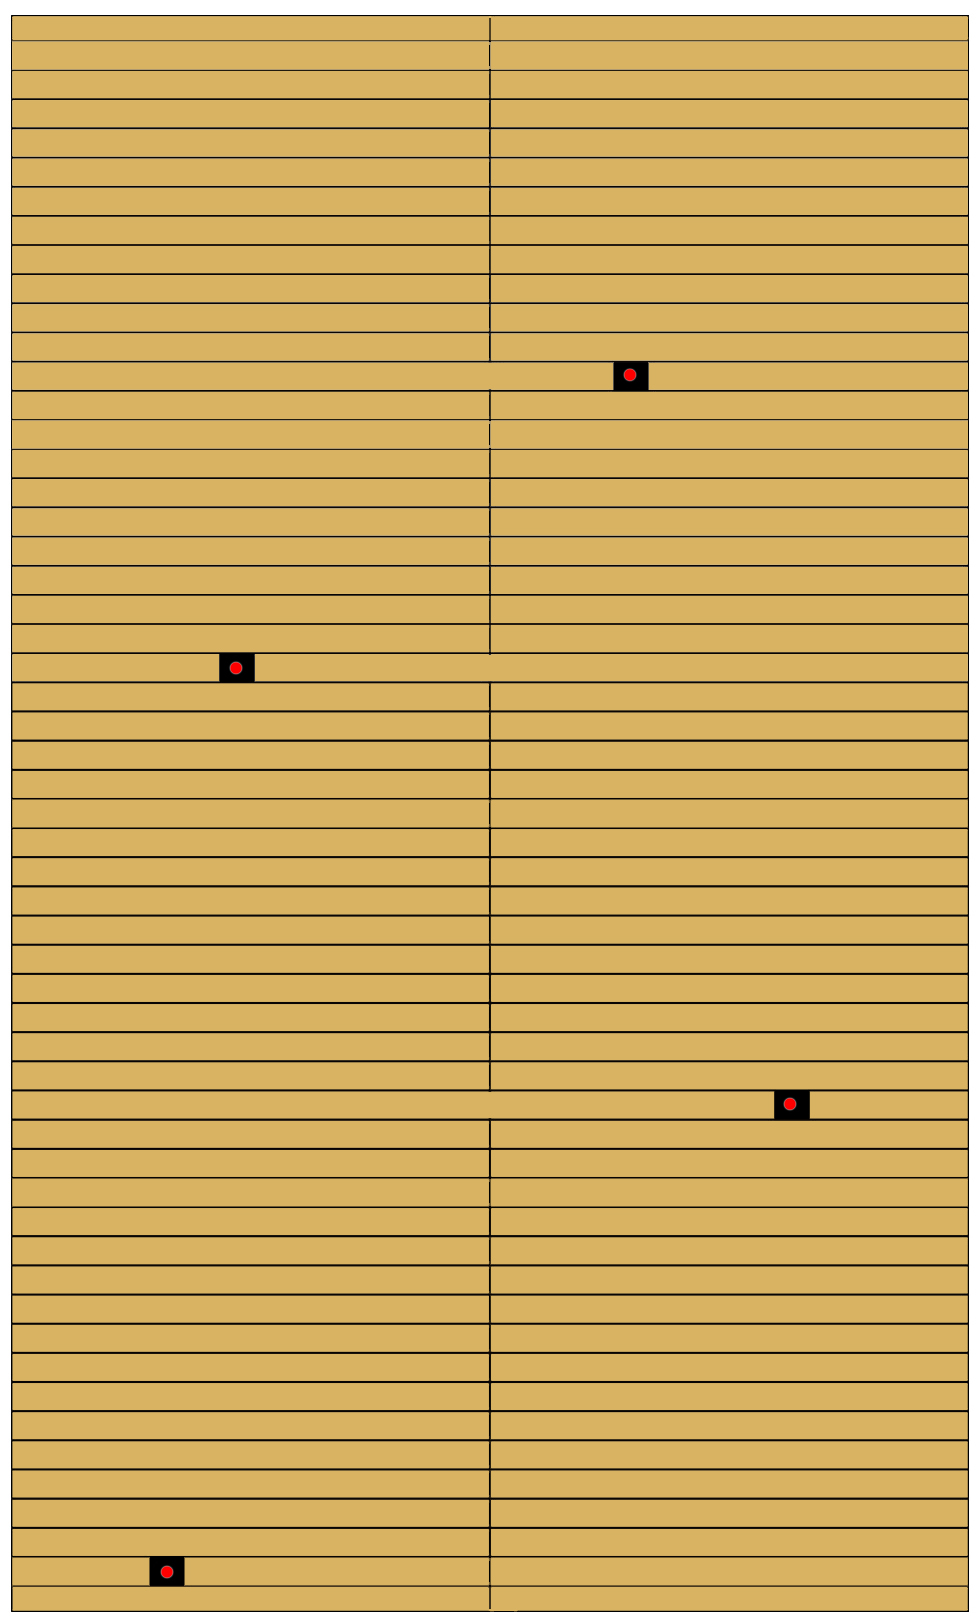
\includegraphics[height=0.8\textheight]{FIGURES/CSU-puntos}
    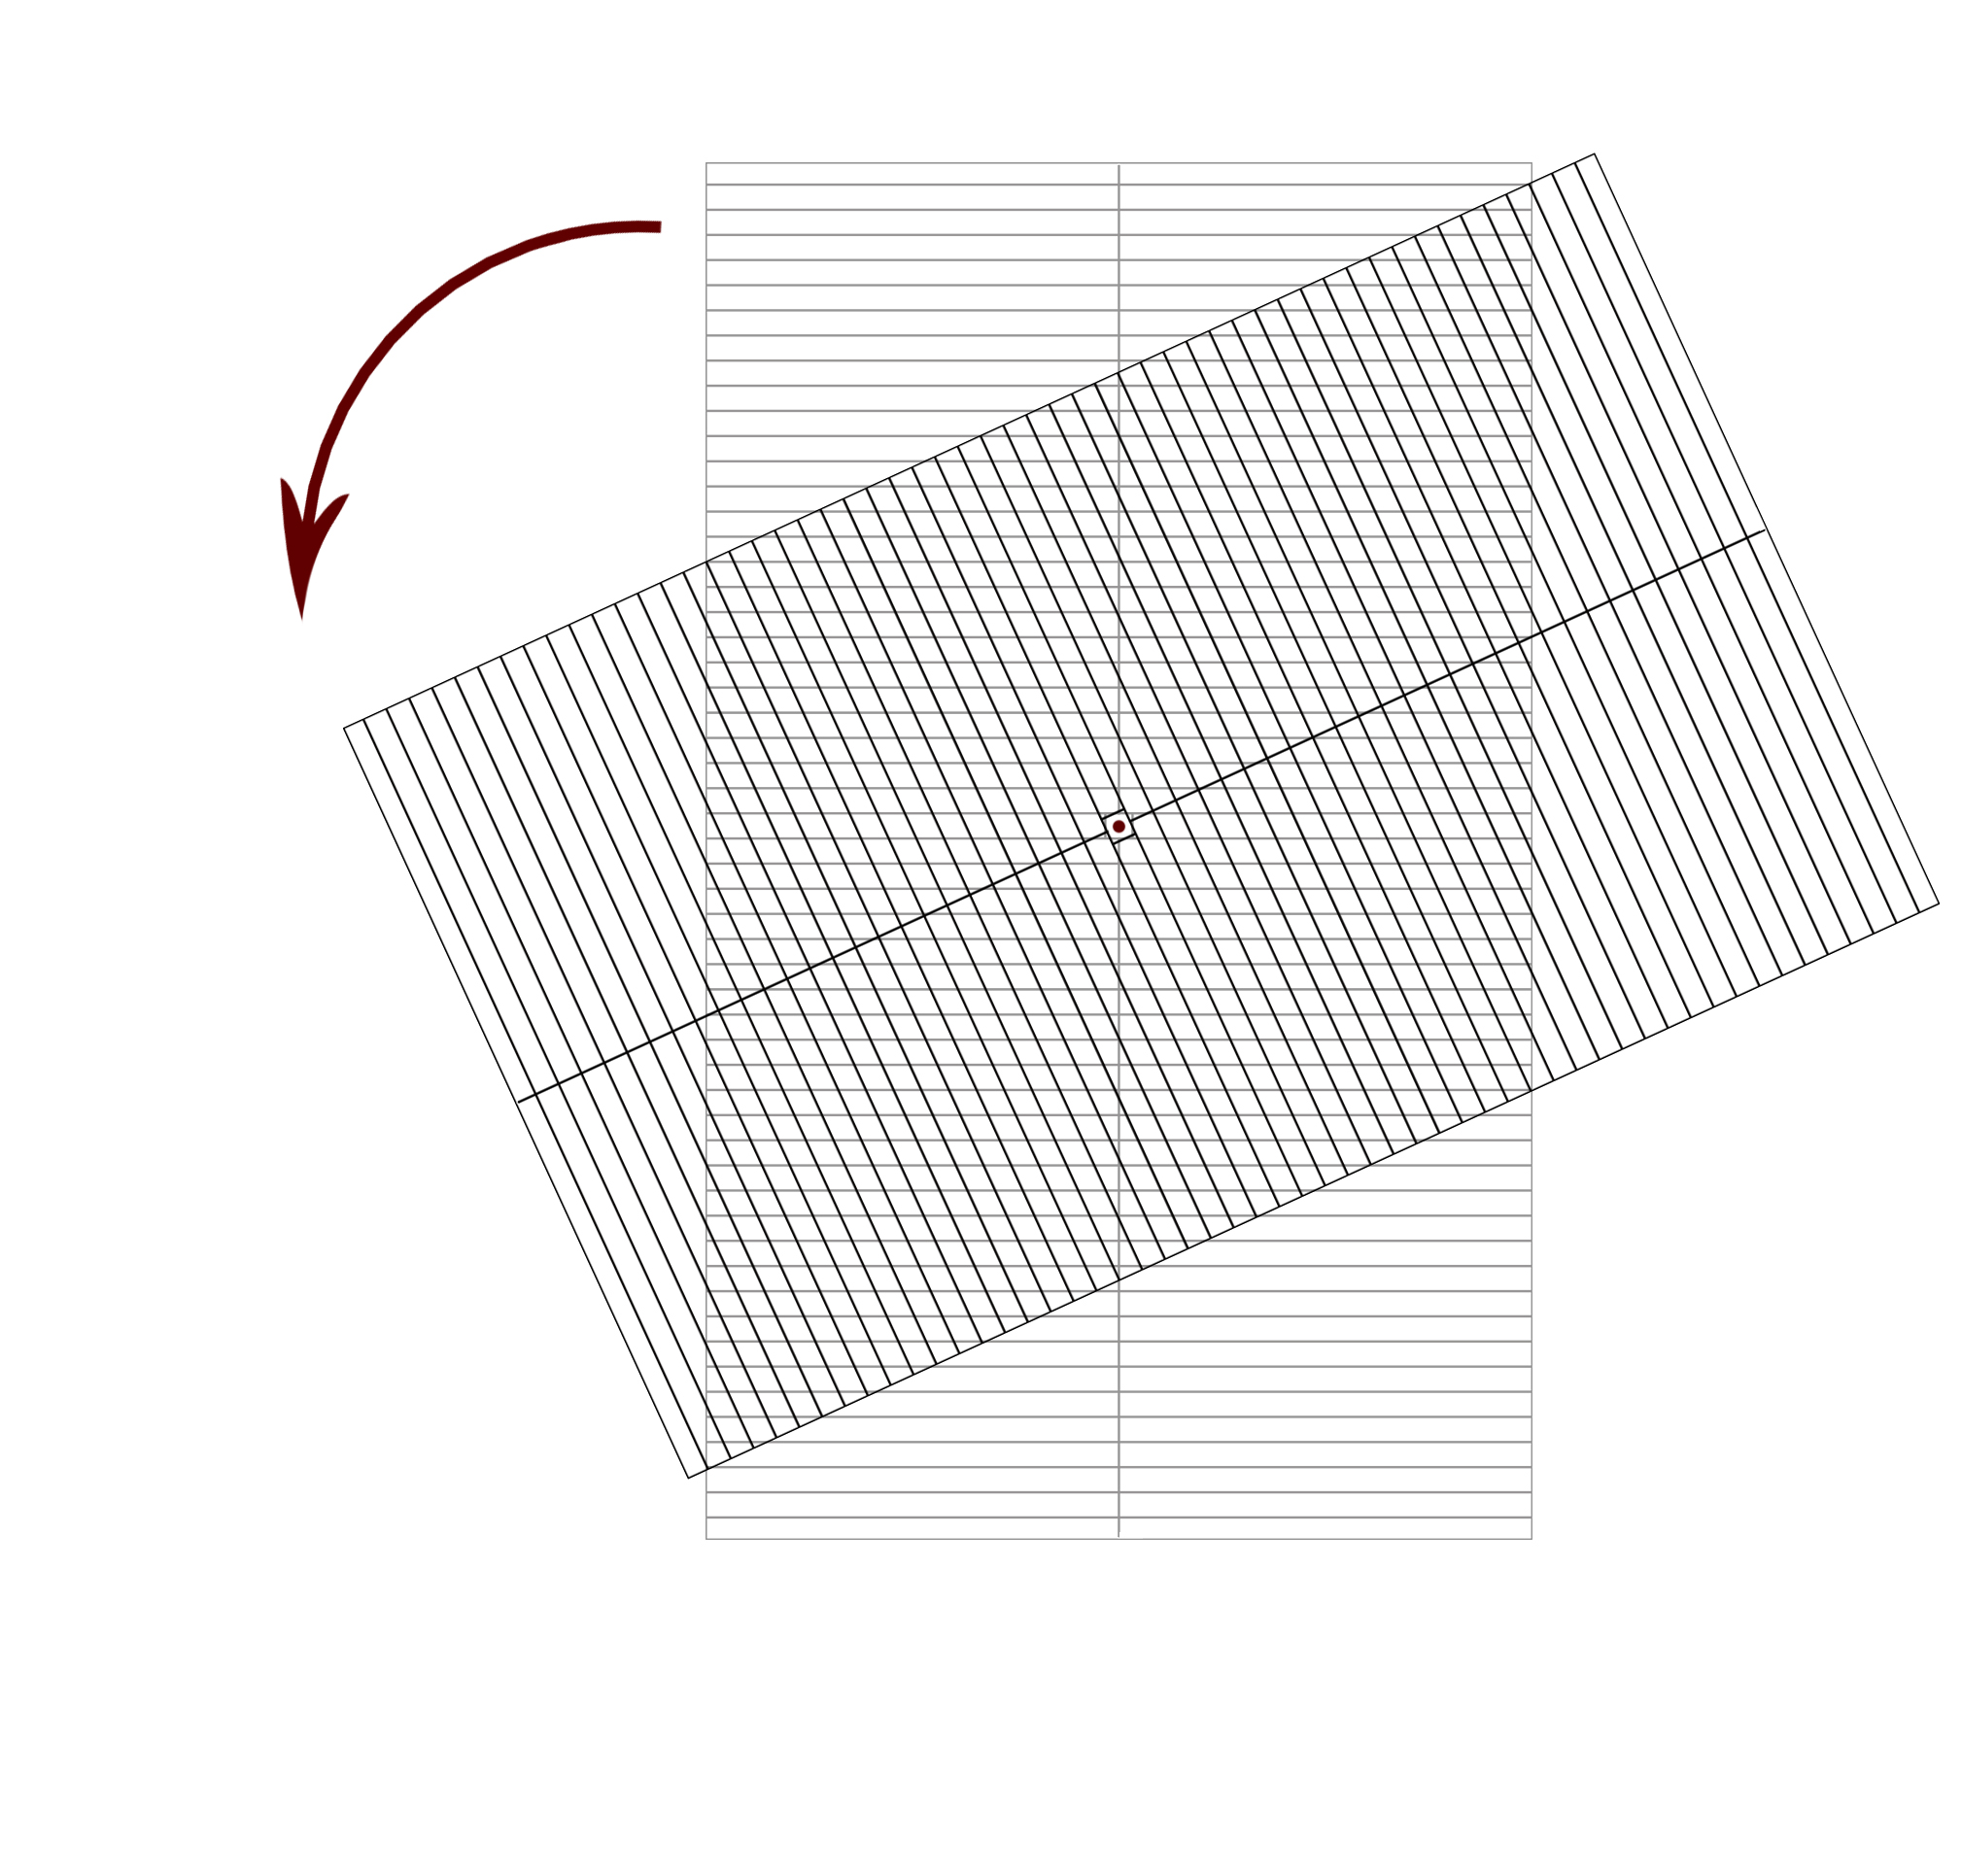
\includegraphics[width=0.7\linewidth]{FIGURES/CSU-giro}
\end{frame}
%%%%%%%%%%%%%%%%%%%%%%%%%%%%%%%%%%%%%%%%%%%%%%%%%%%%%%%%%%%%%%

%%%%%%%%%%%%%%%%%%%%%%%%%%%%%%%%%%%%%%%%%%%%%%%%%%%%%%%%%%%%%%
\begin{frame}
    \frametitle{Problema}
    \centering{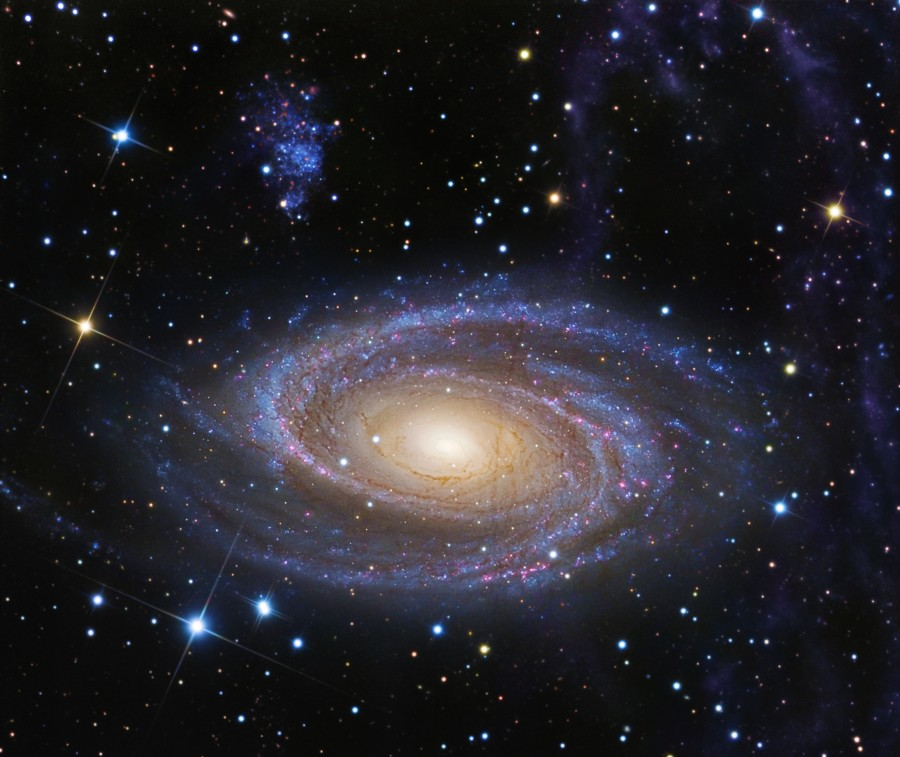
\includegraphics[width=0.6\linewidth]{FIGURES/lrg_ngc3031gabany900c}}
    \block{Descripción}
    \begin{itemize}[<+->]
		\item Número de objetos a observar $>>$ número de barras
    \item Minimizar el tiempo de observación es crítico
    \item Configuración compleja
    \end{itemize}
    \endblock{}
\end{frame}
%%%%%%%%%%%%%%%%%%%%%%%%%%%%%%%%%%%%%%%%%%%%%%%%%%%%%%%%%%%%%%

%%%%%%%%%%%%%%%%%%%%%%%%%%%%%%%%%%%%%%%%%%%%%%%%%%%%%%%%%%%%%%
\begin{frame}
    \frametitle{Objetivos}
    \block{Una aplicación que:}
      \begin{itemize}[<+->]
      \item Resuelva el problema
      \item Minimice el tiempo de respuesta
      \item Contemple prioridades
      \item Contemple Beam Switching
      \end{itemize}
    \endblock{}
\end{frame}
%%%%%%%%%%%%%%%%%%%%%%%%%%%%%%%%%%%%%%%%%%%%%%%%%%%%%%%%%%%%%%

%%%%%%%%%%%%%%%%%%%%%%%%%%%%%%%%%%%%%%%%%%%%%%%%%%%%%%%%%%%%%%
\begin{frame}
    \frametitle{Problema}
    \centering{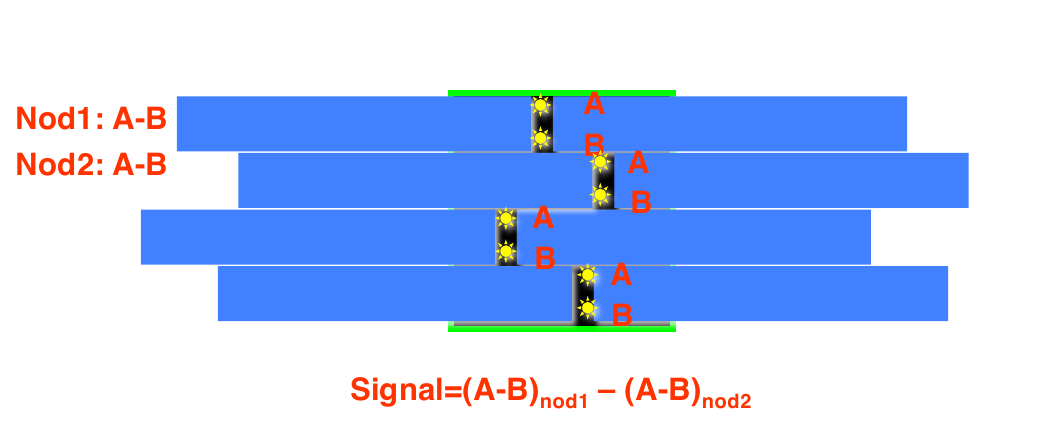
\includegraphics[width=\linewidth]{FIGURES/beamexplication}}
    \block{Beam switching}
		\begin{itemize}
		\item Método para obtener mediciones más precisas
		\item Se mide la luz procedente del objeto y la de la bóveda celeste
		\item Se mueve ligeramente la posición del medidor y se repite la medida
		\end{itemize}
    \endblock{}
\end{frame}
%%%%%%%%%%%%%%%%%%%%%%%%%%%%%%%%%%%%%%%%%%%%%%%%%%%%%%%%%%%%%%

%%%%%%%%%%%%%%%%%%%%%%%%%%%%%%%%%%%%%%%%%%%%%%%%%%%%%%%%%%%%%%
\begin{frame}
    \frametitle{Solución}
    \block{Frentes de actuación}
    \begin{itemize}
		\item Clustering
    \item Algoritmo Constructivo
    \end{itemize}
    \endblock{}
\end{frame}
%%%%%%%%%%%%%%%%%%%%%%%%%%%%%%%%%%%%%%%%%%%%%%%%%%%%%%%%%%%%%%

%%%%%%%%%%%%%%%%%%%% Code  %%%%%%%%%%%%%%%%%%%%%%%%%%%%%%%%%%%
\begin{frame}[fragile]
\frametitle{Clustering}
\block{DBScan}
\endblock{}
%\begin{algorithm}
\begin{lstlisting}[linewidth=\linewidth, mathescape,
numbers=none,basicstyle=\ttfamily\footnotesize]
DBSCAN($D$, $eps$, $MinPts$) {
   $C = 0$
   For(cada punto $P$ no visitado en el cjto de datos $D$) {
      marcar $P$ como visitado
      $NeighborPts =$ regionQuery($P$, $eps$)
      If(sizeof($NeighborPts$) $< MinPts$)
         marcar $P$ como $RUIDO$
      else {
         $C =$ siguiente cluster
         expandCluster($P$, $NeighborPts$, $C$, $eps$, $MinPts$)
      }   
   }   
}
\end{lstlisting}
%\end{algorithm}
\end{frame}
%%%%%%%%%%%%%%%%%%%%%%%%%%%%%%%%%%%%%%%%%%%%%%%%%%%%%%%%%%%%%%

%%%%%%%%%%%%%%%%%%%%%%%%%%%%%%%%%%%%%%%%%%%%%%%%%%%%%%%%%%%%%%
\begin{frame}
    \frametitle{Clustering}
    \block{DBSCAN}
    \endblock{}
		\begin{center}
    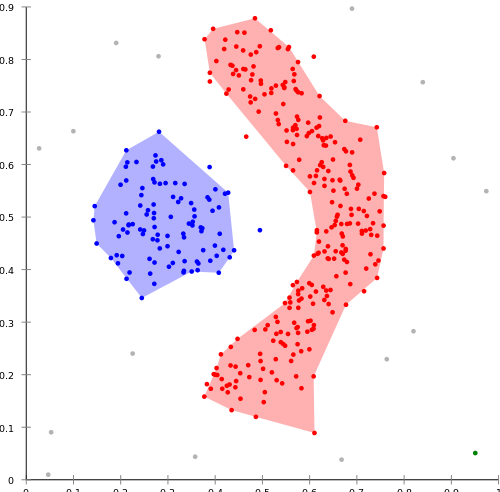
\includegraphics[height=0.8\textheight]{FIGURES/DBSCAN-density-data}
		\end{center}
\end{frame}
%%%%%%%%%%%%%%%%%%%%%%%%%%%%%%%%%%%%%%%%%%%%%%%%%%%%%%%%%%%%%%

%%%%%%%%%%%%%%%%%%%%%%%%%%%%%%%%%%%%%%%%%%%%%%%%%%%%%%%%%%%%%%
\begin{frame}
    \frametitle{Clustering}
    \block{DBSCAN}
    \endblock{}
		\begin{center}
    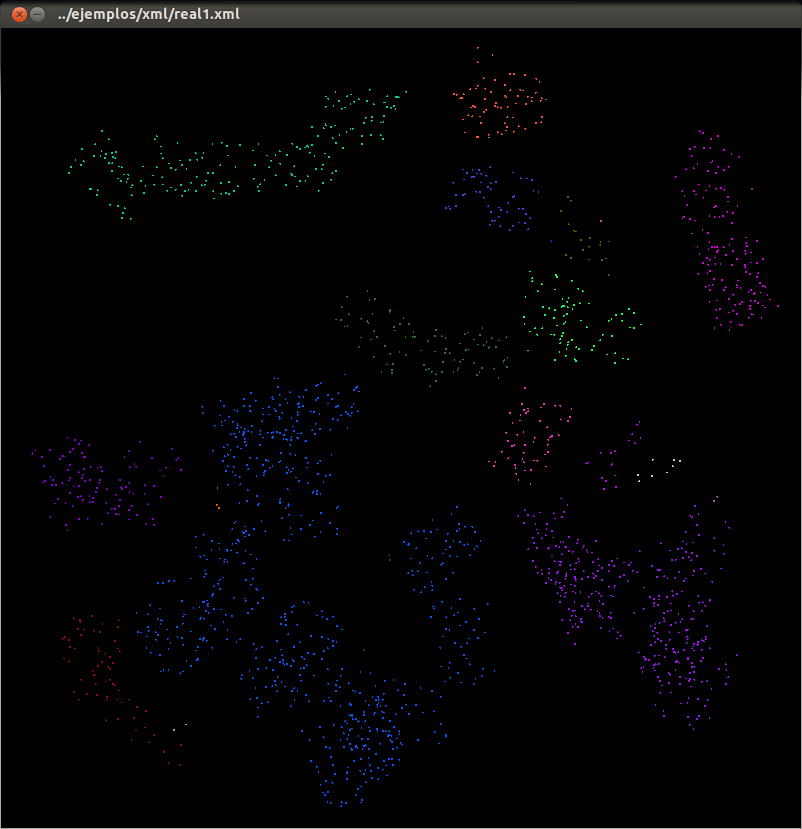
\includegraphics[height=0.8\textheight]{FIGURES/dbscan-e86-m4}
		\end{center}
\end{frame}
%%%%%%%%%%%%%%%%%%%%%%%%%%%%%%%%%%%%%%%%%%%%%%%%%%%%%%%%%%%%%%

%%%%%%%%%%%%%%%%%%%%%%%%%%%%%%%%%%%%%%%%%%%%%%%%%%%%%%%%%%%%%%
\begin{frame}[fragile]
    \frametitle{Solución}
    \block{Algoritmo Constructivo}
    \endblock{}
		\begin{center}
    \begin{lstlisting}[linewidth=\linewidth, mathescape,
    numbers=none,basicstyle=\ttfamily\footnotesize]
For (Cada tipo de ordenacion) {
  ordenar los objetos
  While (queden objetos por cubrir) {
    $p \leftarrow$ siguiente punto de la lista no eliminado
    $C =$ mejor CSU $\in$ crearApuntados($p$, $puntos$)
    puntos -= $\forall$ puntos $\in C$
    Solucion$[tipo orden]  = Solucion$[tipo orden] $\bigcup{C}$
  }
}
$Sol =$ min(Solucion[tipo orden])
    \end{lstlisting}
		\end{center}
\end{frame}
%%%%%%%%%%%%%%%%%%%%%%%%%%%%%%%%%%%%%%%%%%%%%%%%%%%%%%%%%%%%%%

%%%%%%%%%%%%%%%%%%%% Code  %%%%%%%%%%%%%%%%%%%%%%%%%%%%%%%%%%%
\begin{frame}[fragile]
    \frametitle{Algoritmo Constructivo}
    \block{Fase 1: Obtención de objetos}
    \endblock{}
    \begin{lstlisting}[linewidth=\linewidth, numbers=none,basicstyle=\ttfamily\footnotesize]
int estaDentro(const Element &p) const {
  static double new_x, new_y, zone;                            
  if (estaDentro2(p)) {
    testeo(p, new_x, new_y);
    zone = sqrt((Ax - new_x) * (Ax - new_x)i + (Ay - new_y) * (Ay - new_y));
    barra = (int)(zone / DIST_BARRAS);
    if (barra == NUM_BARRAS)
      return 0;
    rango = zone - (barra * DIST_BARRAS);
    distancia = sqrt((p.getx() - new_x) * (p.getx() - new_x) + (p.gety() - new_y) * (p.gety() - new_y));
    if (distancia > 2*ANCHO)
      return 0;
    if (barras_ocupadas[barra])
      return p_potencial(rango, barra);
  }
  return 0;
}
    \end{lstlisting}
\end{frame}
%%%%%%%%%%%%%%%%%%%%%%%%%%%%%%%%%%%%%%%%%%%%%%%%%%%%%%%%%%%%%%

%%%%%%%%%%%%%%%%%%%%%%%%%%%%%%%%%%%%%%%%%%%%%%%%%%%%%%%%%%%%%%
\begin{frame}
    \frametitle{Algoritmo Constructivo}
    \block{Fase 1: Obtención de objetos}
    \endblock{}
		\begin{center}
    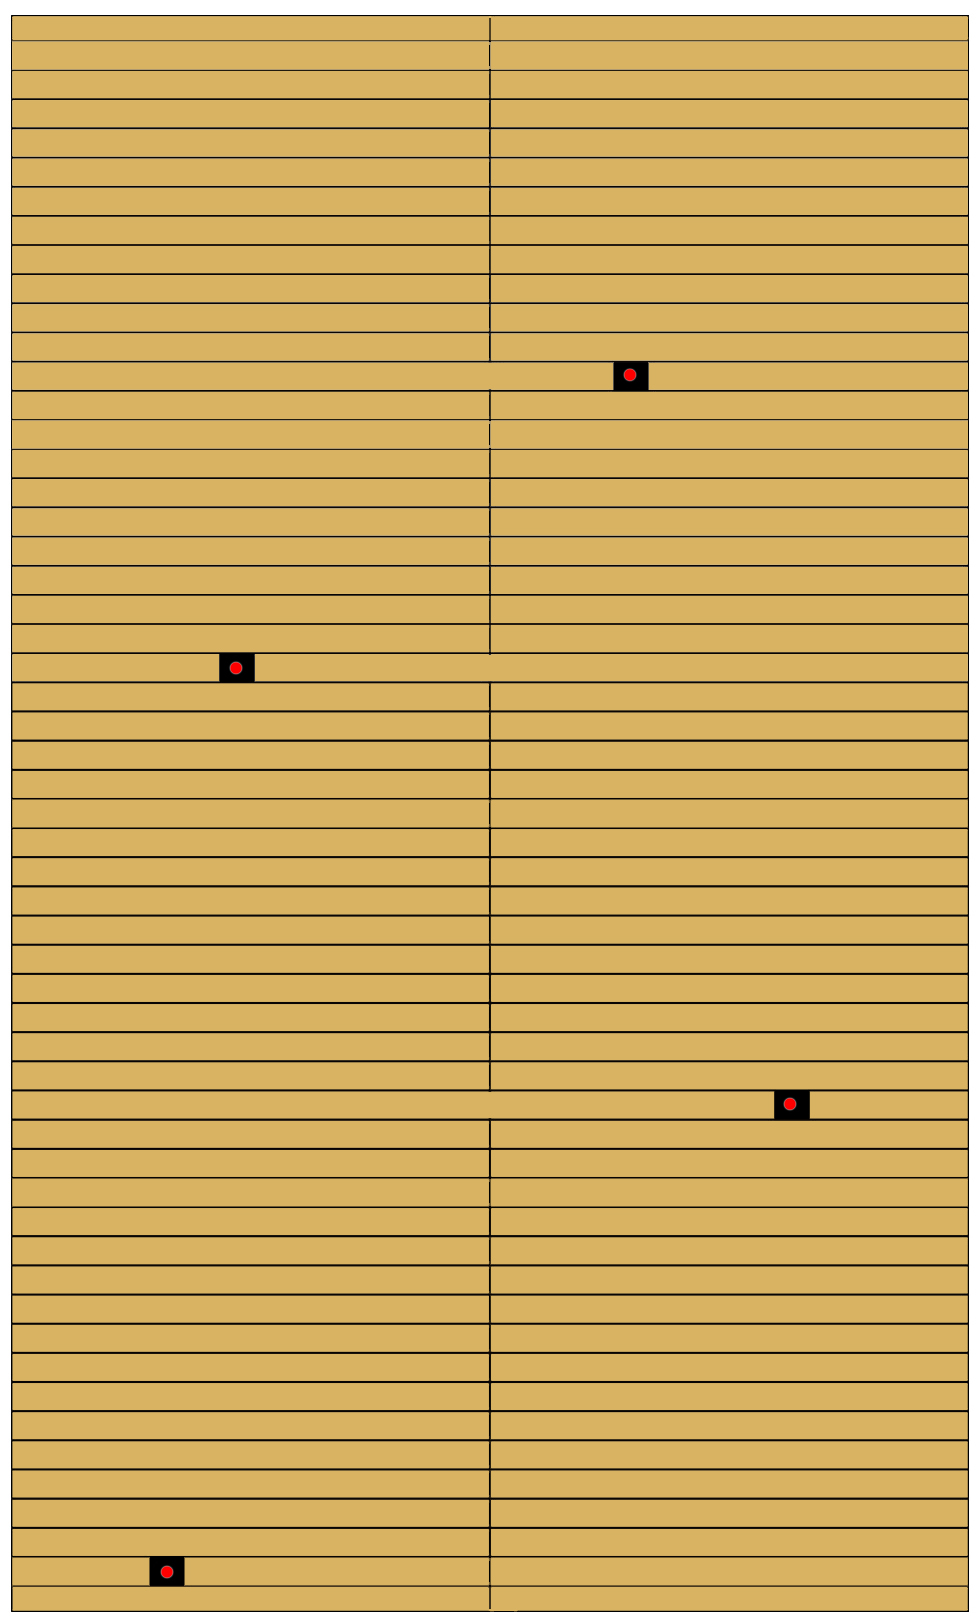
\includegraphics[height=0.8\textheight]{FIGURES/CSU-puntos}
		\end{center}
\end{frame}
%%%%%%%%%%%%%%%%%%%%%%%%%%%%%%%%%%%%%%%%%%%%%%%%%%%%%%%%%%%%%%

%%%%%%%%%%%%%%%%%%%% Code  %%%%%%%%%%%%%%%%%%%%%%%%%%%%%%%%%%%
\begin{frame}[fragile]
    \frametitle{Algoritmo Constructivo}
    \block{Fase 2: Mejora}
    \endblock{}
    \begin{lstlisting}[linewidth=\linewidth, mathescape,
    numbers=none,basicstyle=\ttfamily\footnotesize]
For(Todas las rotaciones posibles) {
    Crear $CSU$ con centro en en el objeto
    rellenar_con_puntos($CSU$, $lista\_objetos$)
    While(numero de puntos en $CSU$ cambie) {
        movimiento de mejora arriba
        rellenar_con_puntos($CSU$, $puntos$)
        movimiento de mejora abajo
        rellenar_con_puntos($CSU$, $puntos$)
        movimiento de mejora izquierda
        rellenar_con_puntos($CSU$, $puntos$)
        movimiento de mejora derecha
        rellenar_con_puntos($CSU$, $puntos$)
    }
    $posibles = posibles \bigcup{CSU}$
}
    \end{lstlisting}
\end{frame}
%%%%%%%%%%%%%%%%%%%%%%%%%%%%%%%%%%%%%%%%%%%%%%%%%%%%%%%%%%%%%%

%%%%%%%%%%%%%%%%%%%%%%%%%%%%%%%%%%%%%%%%%%%%%%%%%%%%%%%%%%%%%%
\begin{frame}
    \frametitle{Algoritmo Constructivo}
    \block{Fase 2: Mejora}
    \endblock{}
		\begin{center}
    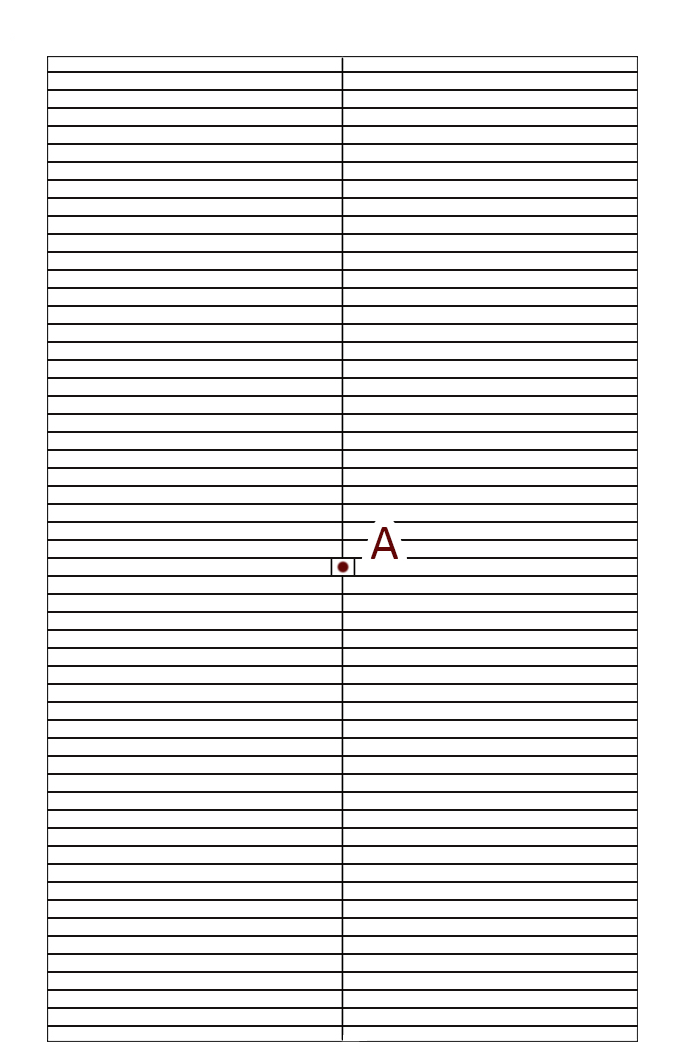
\includegraphics[height=0.8\textheight]{FIGURES/paso1}
		\end{center}
\end{frame}
%%%%%%%%%%%%%%%%%%%%%%%%%%%%%%%%%%%%%%%%%%%%%%%%%%%%%%%%%%%%%%

%%%%%%%%%%%%%%%%%%%%%%%%%%%%%%%%%%%%%%%%%%%%%%%%%%%%%%%%%%%%%%
\begin{frame}
    \frametitle{Algoritmo Constructivo}
    \block{Fase 2: Mejora}
    \endblock{}
		\begin{center}
    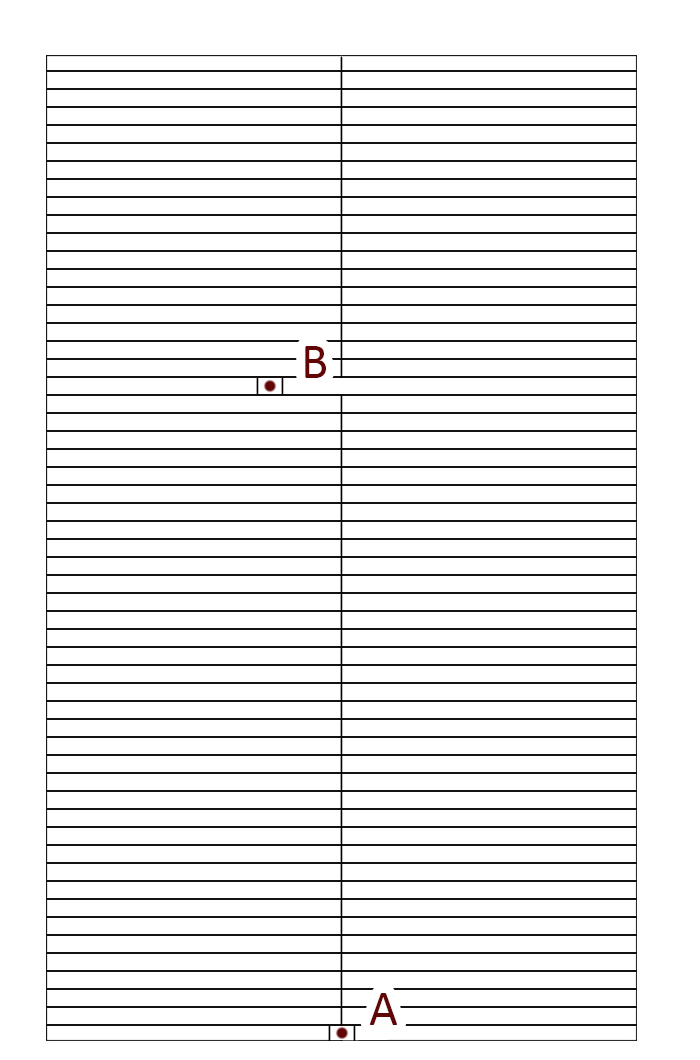
\includegraphics[height=0.8\textheight]{FIGURES/paso2}
		\end{center}
\end{frame}
%%%%%%%%%%%%%%%%%%%%%%%%%%%%%%%%%%%%%%%%%%%%%%%%%%%%%%%%%%%%%%

%%%%%%%%%%%%%%%%%%%%%%%%%%%%%%%%%%%%%%%%%%%%%%%%%%%%%%%%%%%%%%
\begin{frame}
    \frametitle{Algoritmo Constructivo}
    \block{Fase 2: Mejora}
    \endblock{}
		\begin{center}
    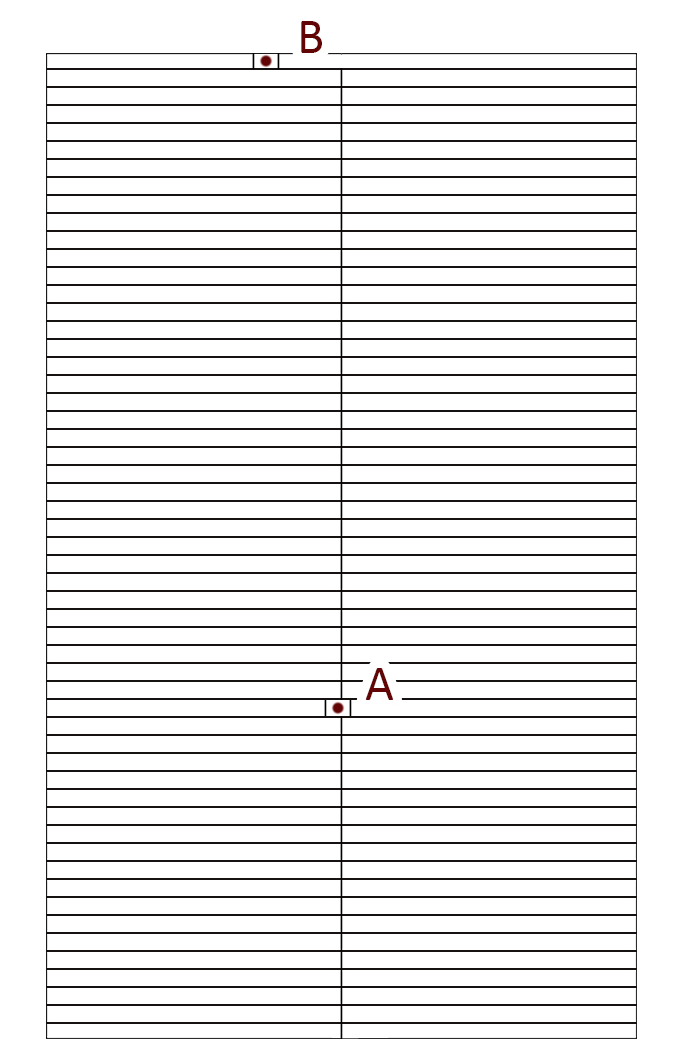
\includegraphics[height=0.8\textheight]{FIGURES/paso3}
		\end{center}
\end{frame}
%%%%%%%%%%%%%%%%%%%%%%%%%%%%%%%%%%%%%%%%%%%%%%%%%%%%%%%%%%%%%%

%%%%%%%%%%%%%%%%%%%%%%%%%%%%%%%%%%%%%%%%%%%%%%%%%%%%%%%%%%%%%%
\begin{frame}
    \frametitle{Algoritmo Constructivo}
    \block{Fase 2: Mejora}
    \endblock{}
		\begin{center}
    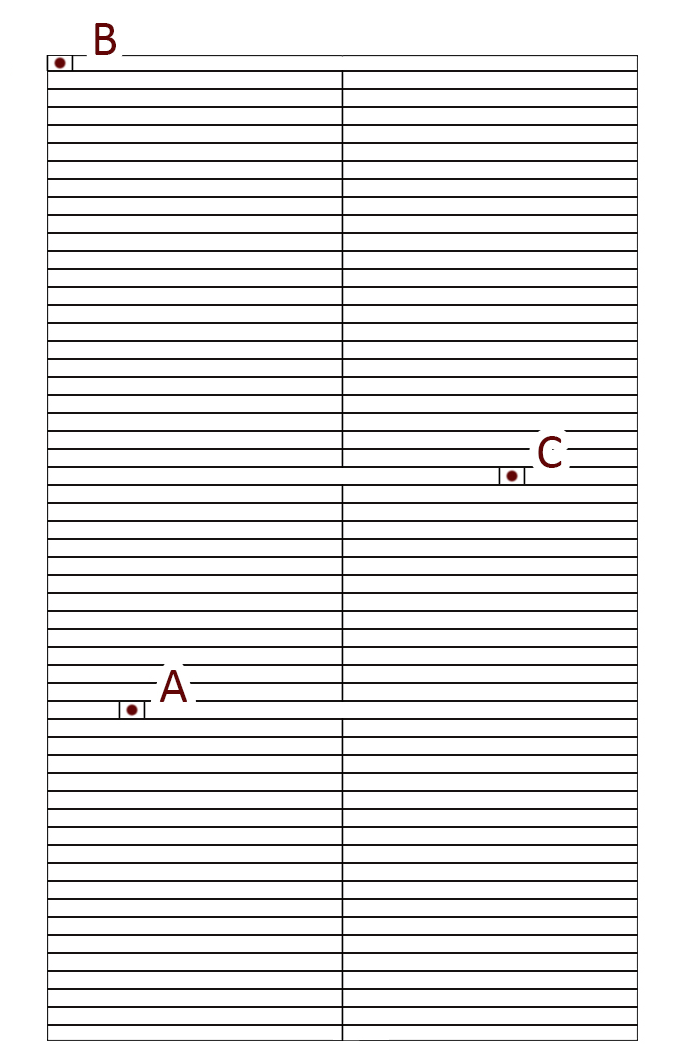
\includegraphics[height=0.8\textheight]{FIGURES/paso4}
		\end{center}
\end{frame}
%%%%%%%%%%%%%%%%%%%%%%%%%%%%%%%%%%%%%%%%%%%%%%%%%%%%%%%%%%%%%%

%%%%%%%%%%%%%%%%%%%%%%%%%%%%%%%%%%%%%%%%%%%%%%%%%%%%%%%%%%%%%%
\begin{frame}
    \frametitle{Algoritmo Constructivo}
    \block{Fase 2: Mejora}
    \endblock{}
		\begin{center}
    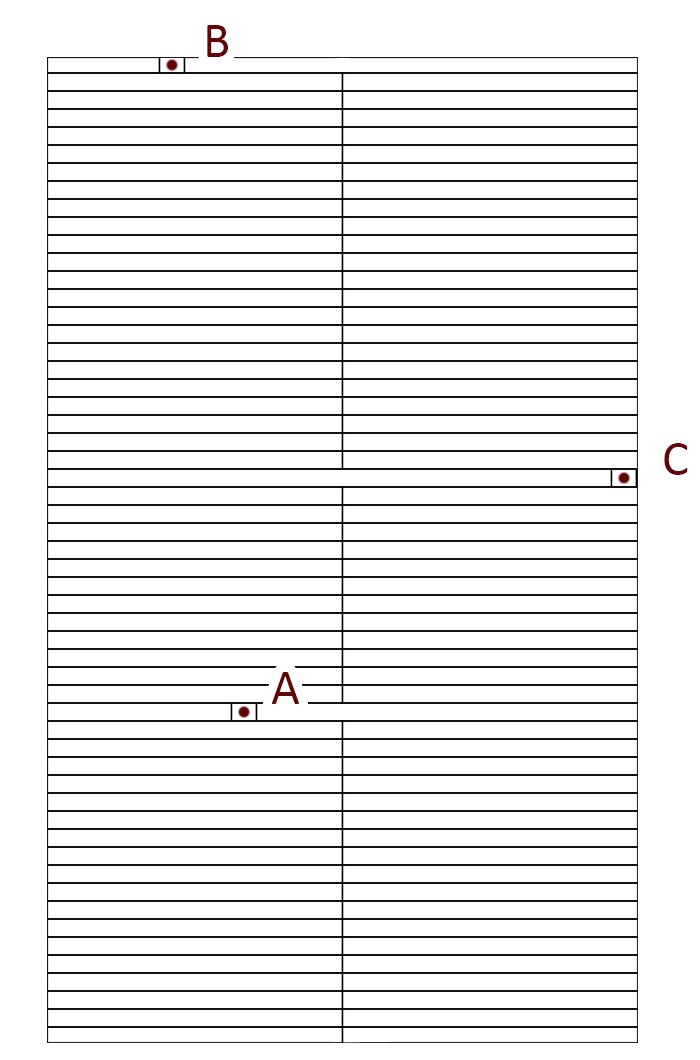
\includegraphics[height=0.8\textheight]{FIGURES/paso5}
		\end{center}
\end{frame}
%%%%%%%%%%%%%%%%%%%%%%%%%%%%%%%%%%%%%%%%%%%%%%%%%%%%%%%%%%%%%%

%%%%%%%%%%%%%%%%%%%%%%%%%%%%%%%%%%%%%%%%%%%%%%%%%%%%%%%%%%%%%%
\begin{frame}
    \frametitle{Obtención de objetos}
    \block{Problema - Colisión}
    \endblock{}
		\begin{center}
    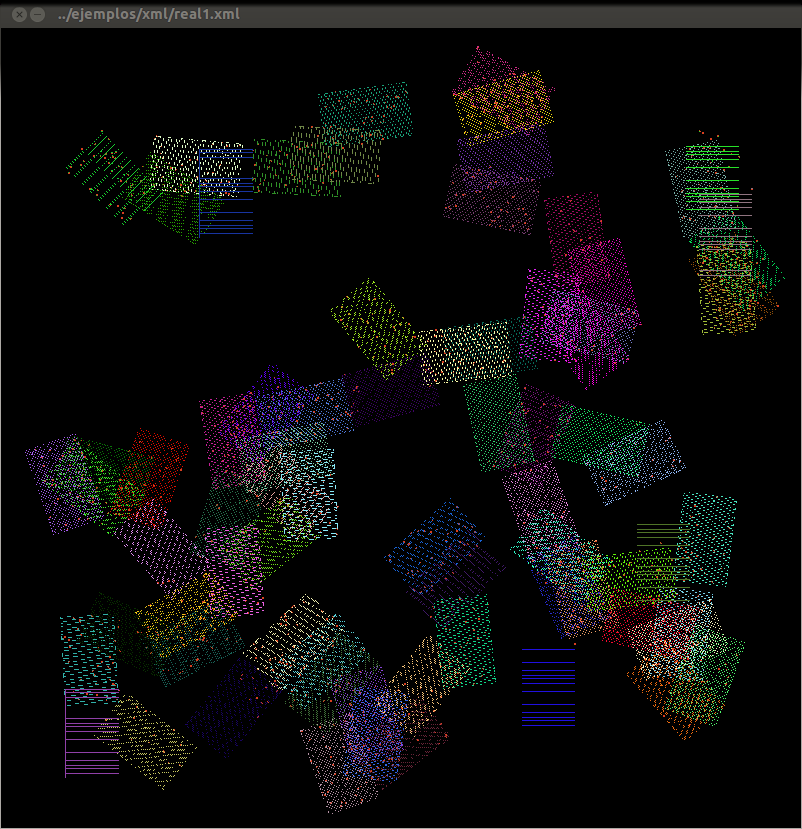
\includegraphics[height=0.8\textheight]{FIGURES/real1-out}
		\end{center}
\end{frame}
%%%%%%%%%%%%%%%%%%%%%%%%%%%%%%%%%%%%%%%%%%%%%%%%%%%%%%%%%%%%%%

%%%%%%%%%%%%%%%%%%%%%%%%%%%%%%%%%%%%%%%%%%%%%%%%%%%%%%%%%%%%%%
\begin{frame}
    \frametitle{Obtención de objetos}
    \block{Problema - Colisión}
    \endblock{}
		\begin{center}
    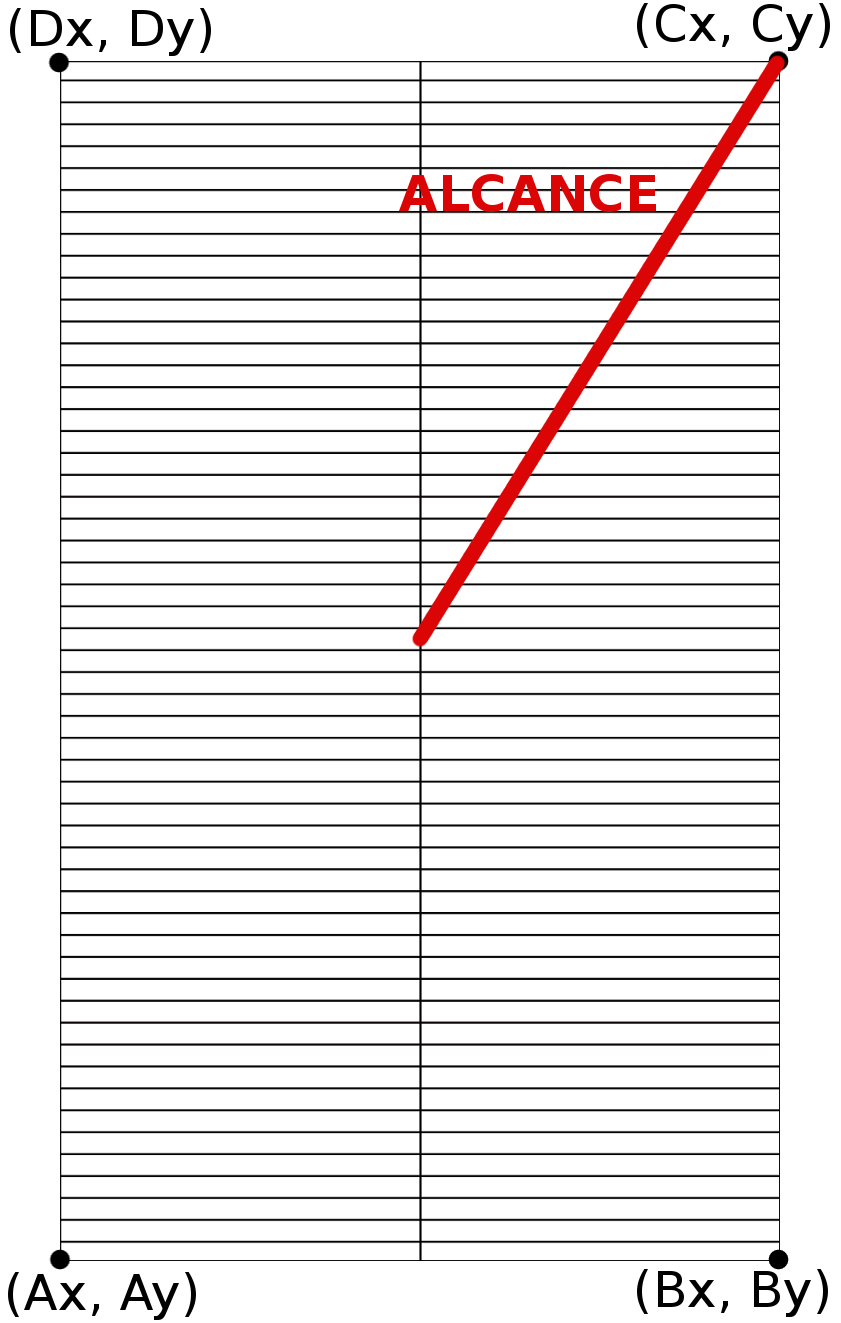
\includegraphics[height=0.8\textheight]{FIGURES/CSU-vertices}
		\end{center}
\end{frame}
%%%%%%%%%%%%%%%%%%%%%%%%%%%%%%%%%%%%%%%%%%%%%%%%%%%%%%%%%%%%%%






%%%%%%%%%%%%%%%%%%%% Code  %%%%%%%%%%%%%%%%%%%%%%%%%%%%%%%%%%%
\begin{frame}[fragile]
\frametitle{Reducción de colisiones}
%\block{}
%\endblock{}
\begin{lstlisting}[linewidth=\linewidth,
mathescape,numbers=none,basicstyle=\ttfamily\scriptsize]
$lista_{ini} =$ resultado
While(Mientras se mejore el resultado) {
    $lista_{fin} =$ los que no colisionan con ninguno.
    While(queden objetos por cubrir) {
        CSU $C \leftarrow$ primer apuntado $\in lista_{ini}$
        $subcto\_puntos = $ puntos de $C$
        Quitar $C$ de $lista_{ini}$
        While(queden CSUs $Q$ por mirar en $lista_{ini}$) {
            If($Q$ colisiona con $C$) {
                $subcto\_puntos += $ puntos de $Q$
                Quitar $Q$ de $lista_{ini}$
            }
        }
        If(colision innecesaria) {
            Obtener_nuevos_apuntados($subcto\_puntos$)
            If(consigue mejorar) 
              $lista_{ini} +=$ nuevos apuntado  
            else {
              Introducir en $lista_{ini}$ los que se quitaron
              Poner en $lista_{fin}$ el apuntado $C$
            }
        }
    }
    $lista_{ini} = lista_{fin}$
\end{lstlisting}
\end{frame}
%%%%%%%%%%%%%%%%%%%%%%%%%%%%%%%%%%%%%%%%%%%%%%%%%%%%%%%%%%%%%%

